\def\currentRootFolder{chapter/energyDependentCrossSec}
\def\currentFigureFolder{\currentRootFolder/fig}
\newcommand{\sigmaInel}{\sigma_\mathrm{inel}}
\newcommand{\sigmaAvg}{\sigma_\mathrm{avg}}

\newcommand{\qUmin}{qU_\mathrm{min}}

\newcommand{\Ekin}{E_\mathrm{kin}}
\newcommand{\nSource}{n_\mathrm{S}}
\newacronym{standardmodel}{SM}{Standard Model of Particle Physics}
\newacronym{lep}{LEP}{Large Electron Positron Collider}
\newacronym{ssm}{SSM}{standard solar model}
\chapter{Energy-Dependence of the Cross Section for Inelastic Electron Scattering within the \glsentryshort{wgts}}
\label{sec:eDepScatCrossSec}
The probability of an electron to scatter when traveling through the \gls{wgts} can be characterized by the total scattering cross section $\sigma_\mathrm{tot}$. Two types of scatterings can be distinguished: elastic and inelastic scattering. The cross section for elastic scattering is by smaller than the one for inelastic scattering by one order of magnitude~\cite{Kleesiek2019}. This chapter focuses on inelastic scattering and neglects the other. Within this chapter, the cross section for electrons scattering inelastically off tritium molecules is just denoted as ``cross section'' and with the symbol $\sigma$. For ease of notation and reading, the adjective ``inelastic'' and an index such as ``inel'' is omitted where the context allows it unambiguously.

The cross section depends on the energy of the incident electrons: $\sigma \equiv \sigma(\Ekin)$. This dependence has been neglected in the formal modeling of a KATRIN measurement within the previous chapter~\ref{sec:intSpecModel}. This chapter investigates effects related to the incorporation of the energy dependence. Section~\ref{sec:eDepScatCrossSecSources} lists cross section values from different sources and relates them to each other. Section~\ref{sec:eDepScatCrossSecModel} extends the mathematical formalism for a KATRIN measurement in order to incorporate the energy dependence of the scattering cross section. Section~\ref{sec:eDepScatCrossSecNuMassInf} discusses the energy-dependence within the context of neutrino mass inference. In the end, section~\ref{sec:eDepScatCrossSecConclusion} concludes and offers an outlook.


\section{Cross Section for Electrons Scattering off Molecules of Hydrogen Isotopologues}
\label{sec:eDepScatCrossSecSources}
There exist several sources for cross-section formulae and values. This section gives an overview about the sources considered in this thesis and how they relate to each other. First, the cross section for electrons with an energy of \SI{18600}{eV} scattering off tritium was measured at the Troitsk experiment to be~\cite{Aseev2000}
\begin{equation}
	\sigma(\SI{18600}{eV}) = \SI{3.40\pm0.07e-22}{m^{-22}} \fullstop
\end{equation}
Also, the KATRIN Design Report lists a reference value~\cite{Angrik:2005ep}
\begin{equation}
	\sigma_\mathrm{TDR} = \SI{3.456e-22}{m^{-2}} \fullstop
\end{equation}
Furthermore, there exist theoretical calculations of the cross section for electrons scattering of hydrogen molecules. In section~\ref{sec:eDepScatCrossSecSourcesTheory} the theoretical formulae are reviewed. How the different sources relate to each other and what approach is chosen within the scope of this thesis is explained in section~\ref{sec:eDepScatCrossSecSourcesChoice}.
\subsection{Theoretical Formulae}
\label{sec:eDepScatCrossSecSourcesTheory}
An expression for the inelastic cross section for electrons scattering from hydrogen molecules can be found in~\cite{Liu1973}. Two expressions are given, one for relativistic incident electrons and one for non-relativistic incident particles. With regard to KATRIN the energies of $\upbeta$ electrons from tritium $\upbeta$ decay are relevant. The maximum relativistic $\beta$ factor of electrons from tritium $\upbeta$ decay is
\begin{align}
\beta(\Ekin, m) &= 
\sqrt{
	1-\frac{1}{
		(\frac{\Ekin}{m}+1)^2
	}
} \label{eq:eDepScatCrossSecSourcesCrossSecBetaFactor} \\
\Rightarrow\beta_\mathrm{max, T} &= 
\beta(\Eeff\approx\SI{18.6}{keV}, m_\elecIndex\approx\SI{511}{keV})\approx0.26 
\fullstop
\end{align}
Traveling at approximately a forth of the speed of light, the $\upbeta$ electrons are assumed to behave non-relativistic. Then, the given expression for the energy dependent cross section is~\cite{Liu1973}
\begin{equation}
\label{eq:eDepScatCrossSecSourcesCrossSecLiu}
\sigma(E) =  
(4 \pi a_0^2) \cdot
\left(\frac{E}{R}\right)^{-1} \cdot
\left[
C_1 \cdot \ln{\left(\frac{E}{R}\right)} + C_2
\right]
\end{equation}
with the Bohr radius\footnote{Bohr radius $a_0=\SI[separate-uncertainty=false]{0.529 177 210 67(12)e-10}{m}$~\cite{ReviewOfParticlePhysics}} $a_0$, 
the Rydberg energy\footnote{Rydberg energy $R=\SI[separate-uncertainty=false]{13.605 693 009(84)}{eV}$~\cite{ReviewOfParticlePhysics}} $R$ and two constants $C_1$ and $C_2$. The later two depend on the hydrogen isotopologue. Different values a stated in different works for isotopic hydrogen
\begin{subequations}
\label{eq:eDepScatCrossSecSourcesCrossSecLiuConstants}
\begin{align}
C_1 &= 1.5487 &&\text{\cite{Liu1973}}
\label{eq:eDepScatCrossSecSourcesCrossSecLiuConstantsC1}\\[10pt]
C_2 &= 2.2212\pm0.0434 &&\text{\cite{Liu1973}}
\label{eq:eDepScatCrossSecSourcesCrossSecLiuConstantsC2Uncert}\\
C_2 &= 1.53 &&\text{\cite{Gerhart1975}} \\
C_2 &= 2.4036 &&\text{\cite{Liu1987}}
\label{eq:eDepScatCrossSecSourcesCrossSecLiuConstantsC2}
\fullstop
\end{align}
\end{subequations}
The latest of these references~\cite{Liu1987} acknowledges that the listed values for $C_2$ are not compatible. Within this work, the value from~\cite{Liu1987} is chosen as it is the most up-to-date of the listed ones. 

In equation~\eqref{eq:eDepScatCrossSecSourcesCrossSecLiu}, $E$ denotes\footnote{I would like to thank F. Glück for pointing this out.}
\begin{equation}
	\label{eq:eDepScatCrossSecSourcesCrossSecNonRelEnergy}
	E \equiv E(\Ekin) = \frac{1}{2} m_\elecIndex \beta^2(\Ekin, m_\elecIndex)
\end{equation}
with $\beta$ as in equation~\eqref{eq:eDepScatCrossSecSourcesCrossSecBetaFactor}. Figure~\ref{fig:eDepScatCrossSecSourcesValues} shows the theoretical cross-section formula along with the measured value by the Troitsk experiment and the value from the KATRIN Design Report.
\begin{figure}[t]
	\centering
	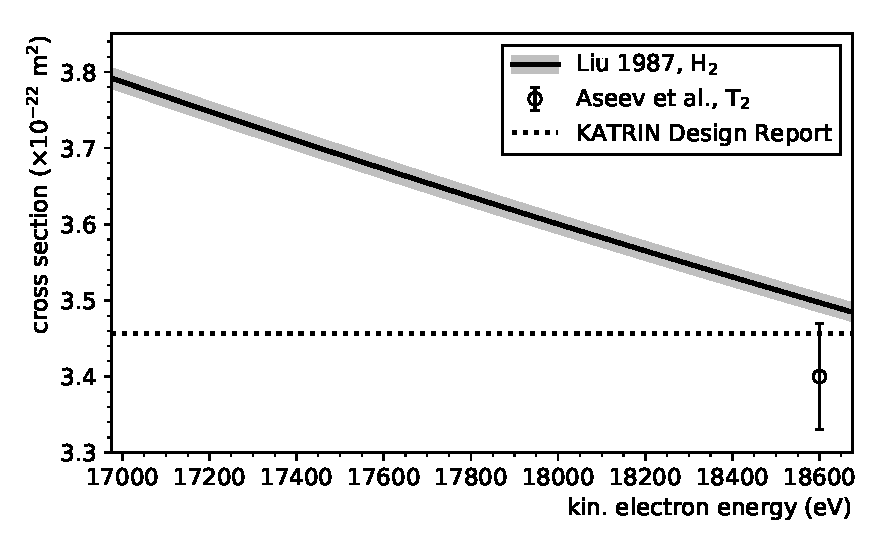
\includegraphics[width=\textwidth]{\currentFigureFolder/crossSecNoZoom.pdf}
	\xcaption{Inelastic cross section for non-relativistic incident electrons scattering off molecular hydrogen isotopologues}{Inelastic cross section for non-relativistic incident electrons scattering off molecular hydrogen isotopologues.}{Shown is the theoretical calculation according to equation~\eqref{eq:eDepScatCrossSecSourcesCrossSecLiu} with constants from equation~\eqref{eq:eDepScatCrossSecSourcesCrossSecLiuConstantsC1} and~\eqref{eq:eDepScatCrossSecSourcesCrossSecLiuConstantsC2} where the later is assumed to have an uncertainty according to equation~\eqref{eq:eDepScatCrossSecSourcesCrossSecLiuConstantsC2Uncert}. Also shown is the measurement by~\cite{Aseev2000} at the Troitsk experiment and the value stated in the KATRIN Design Report~\cite{Angrik:2005ep}. The shown energy interval is chosen according to the \gls{mtd} of the \gls{ft} measurement campaign.}
	\label{fig:eDepScatCrossSecSourcesValues}
\end{figure}

\subsection{Relation to Former Works}
\label{sec:eDepScatCrossSecSourcesChoice}
As can be seen in figure~\ref{fig:eDepScatCrossSecSourcesValues}, the cross section from the KATRIN Design Report does not match the theoretical calculations used in this thesis. However, the value stated in the KATRIN Design Report can be recovered from equation~\eqref{eq:eDepScatCrossSecSourcesCrossSecLiu}. If instead of the energy interpretation
of equation~\ref{eq:eDepScatCrossSecSourcesCrossSecNonRelEnergy}, one applies 
\begin{equation}
	\label{eq:eDepScatCrossSecSourcesCrossSecTDREngeryInterpretation}
	E \equiv \Ekin
	\fullstop
\end{equation}
The obtained cross section is $\sigma(\Ekin \approx \SI{18564.4}{eV}) = \SI{3.456e-22}{m^2}$ as stated in the KATRIN Design Report where the energy \SI{18564.4}{eV} is within the KATRIN design analysis interval (see section~\ref{sec:intSpecModelMTD}). This work applies the energy interpretation~\eqref{eq:eDepScatCrossSecSourcesCrossSecTDREngeryInterpretation} when comparability to former work is of importance. Otherwise, interpretation~\eqref{eq:eDepScatCrossSecSourcesCrossSecNonRelEnergy} is used\footnote{The cross sections obtained from the theoretical formula~\eqref{eq:eDepScatCrossSecSourcesCrossSecLiu} applying the energy interpretation via equation~\eqref{eq:eDepScatCrossSecSourcesCrossSecNonRelEnergy} are in better agreement with recently taken data at KATRIN according to preliminary analysis results by dedicated subgroups of the KATRIN collaboration at the time of writing this thesis.}. Corresponding indications are given.
    
\section{An Energy-Dependent Scattering Model within the KATRIN Formalism}
\label{sec:eDepScatCrossSecModel}
The energy-dependence of the cross section enters into the calculation of the scattering probabilities~\eqref{eq:intSpecModelNonAveragedScatProbs}. In the derivation, that is given in the previous section~\ref{sec:intSpecModelResponseScattering}, the dependence on the starting energy $\Esource$ of electrons is neglected. Instead an average starting energy and hence, an average scattering cross section $\sigma(\SI{18564.4}{eV})=\SI{3.456e-22}{m^2}$ (energy interpretation by the KATRIN Design Report) is assumed. Table~\ref{tab:eDepScatCrossSecModelScatProbs} lists the corresponding scattering probabilities averaged over all starting positions and pitch angles of electrons. Additionally, the results of a Monte-Carlo simulation by~\cite{Groh2015} and the values using the energy interpretation of equation~\eqref{eq:eDepScatCrossSecSourcesCrossSecNonRelEnergy} are given. How the energy-dependence of the scattering probabilities can be modeled is shown in section~\ref{sec:eDepScatCrossSecModelDescription}. Section~\ref{sec:eDepScatCrossSecModelDiscussion} discusses the given model from a physical perspective and section~\ref{sec:eDepScatCrossSecModelPerformanceAndAccuracy} considers its computational performance and accuracy. \todo{update and complete!}

\begin{table}[t]
	\centering
	\xcaption{Probabilities for severalfold scattering of electrons in the \gls{wgts}}{Probabilities for severalfold scattering of electrons in the \gls{wgts}}{averaged over all starting positions and starting pitch angles. Both, the values from a Monte Carlo (MC) simulation and the values according to equation~\eqref{eq:intSpecModelAveragedScatProbs} are given. The  cross section was evaluated at an energy of $E\approx\SI{18764.4}{eV}$
	for the two interpretations described by equation~\eqref{eq:eDepScatCrossSecSourcesCrossSecTDREngeryInterpretation} and~\eqref{eq:eDepScatCrossSecSourcesCrossSecNonRelEnergy}. Further input parameters to the calculations are a constant gas column density $\rho d = \SI{5e17}{cm^{-2}}$, 
	a \gls{wgts} length of $d=\SI{10.0820}{m}$
	and a maximum acceptance angle of $\thetaMax=\SI{50.7685}{\degree}$.}
	\begin{tabular}{lllr}
		\toprule
		\makecell[tl]{cross section (\SI{e-22}{m^{-2}}) $\rightarrow$} &
		3.456 &
		3.456 &
		3.673 \\
		\hline
		\makecell[tl]{source $\rightarrow$} & 
		\makecell[tl]{MC particle tracking\\ \cite{Groh2015}} & 
		\makecell[tl]{eq. \eqref{eq:intSpecModelAveragedScatProbs} \\ \cite{Groh2015, Kleesiek2014}} &
		\makecell[tr]{eq. \eqref{eq:intSpecModelAveragedScatProbs}}
		\\
		\hline
		\makecell[cl]{scattering count $\downarrow$} & 
		& 
	    & \\
		\hline
		\makecell{0} & $0.415 \pm 0.002$ & 0.41334 & 0.39564 \\
		\makecell{1} & $0.292 \pm 0.002$ & 0.29266 & 0.28967 \\
		\makecell{2} & $0.166 \pm 0.001$ & 0.16733 & 0.17298 \\
		\makecell{3} & $0.079 \pm 0.001$ & 0.07913 & 0.08590 \\
		\makecell{4} & $0.031 \pm 0.001$ & 0.03178 & 0.03634 \\
		\bottomrule
	\end{tabular}
	\label{tab:eDepScatCrossSecModelScatProbs}
\end{table}


\subsection{Model Description}
\label{sec:eDepScatCrossSecModelDescription}
\begin{figure}[th]
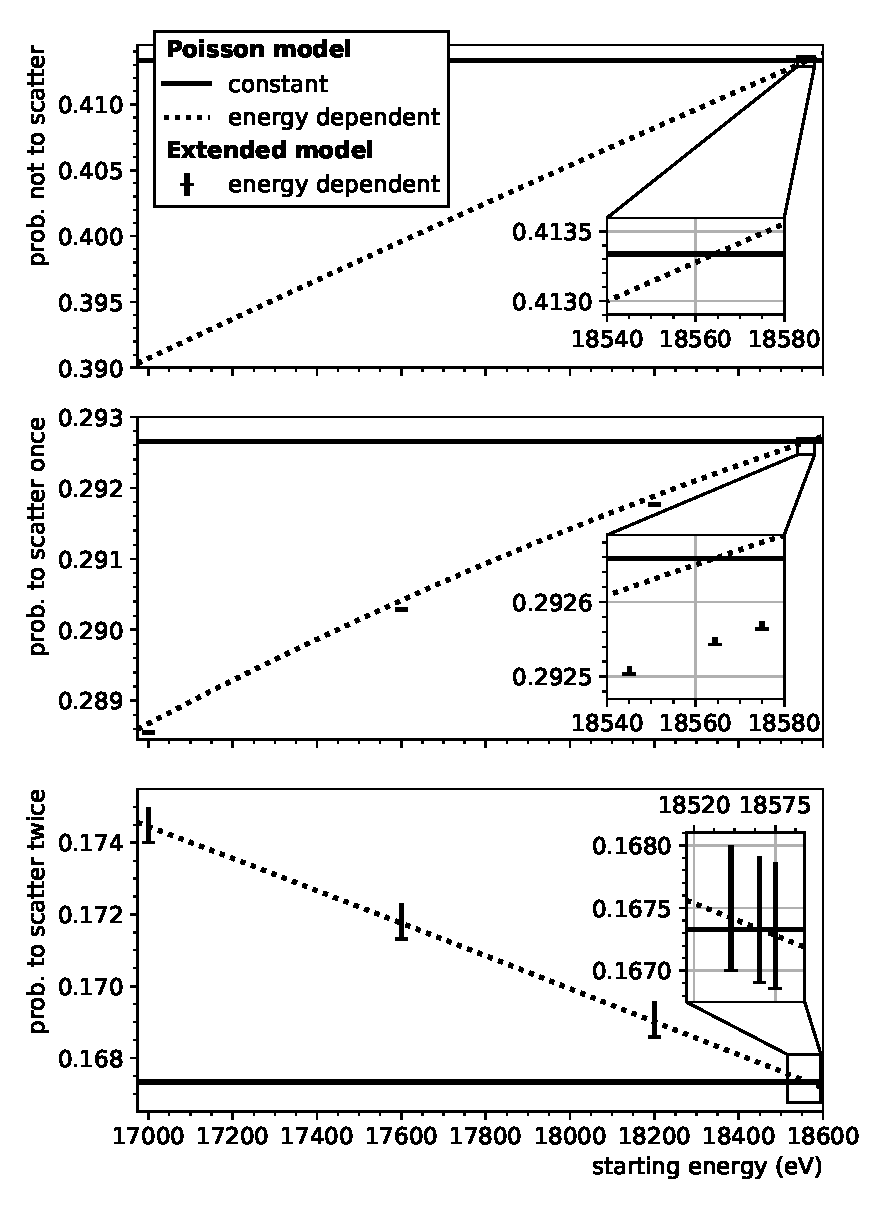
\includegraphics[width=\textwidth]{\currentFigureFolder/scatProbs123.pdf}
        \xcaption{Energy-dependent probability of electron scattering within the \gls{wgts}}{Energy-dependent probability of electron scattering within the \gls{wgts}.}{Shown are from top to bottom the probability for no, 1-fold and 2-fold scattering averaged over all starting positions and starting pitch angles of $\upbeta$ electrons. Depending on the required accuracy, for 1-fold and 2-fold scattering the Poisson model does not hold. The markers show an extended model as described in the text. Its numerical evaluation suffers from a one-sided uncertainty (of $\sim10^{-5}$ for 1-fold and $\sim10^{-3}$ for 2-fold scattering) depicted as uncertainty bars. The inset shows an energy span around the endpoint of the tritium $\upbeta$ spectrum. The full energy range matches the measurement interval of the \glsentryfull{ft} campaign.}
        \label{fig:eDepScatCrossSecModel}
\end{figure}
Within this section, two models are presented in order to incorporate the energy-dependence of the scattering cross section into the mathematical formalism of a KATRIN measurement.

\paragraph{Poisson Model}
An expression for the probability of $l$-fold scattering of electrons within the \gls{wgts} is derived in the previous section~\ref{sec:intSpecModelResponseScattering}. The given model is independent of the energy of the electrons. Instead of using a constant cross section, the energy dependence can be respected. The corresponding formulae from section~\ref{sec:intSpecModelResponseScattering} are repeated below, with the energy-dependence made explicit
\begin{subequations}
\label{eq:energydepScatProbsPoissonModel}
\begin{align}
    \mu(\Esource,\zSource,\thetaSource) =&
    \frac{\sigma(\Esource)}{\cos\thetaSource}
    \int_{\zSource}^{L/2} \rho(z)\d z \label{eq:energydepScatProbsPoissonExpectedScatCount} \\
    P_l(\Esource,\zSource,\thetaSource) =&
    \mathrm{Poisson}(\mu(\Esource,\zSource,\thetaSource),l) \label{eq:nonAveragedEnergydepScatProbsPoisson} \\
    \bar{P}_l(\Esource) =&
    \frac{1}{L \cdot (1-\cos(\thetaMax))} 
      \int_{-L/2}^{L/2}  
          \int_{0}^{\theta_{max}} 
            \sin(\thetaSource)
            \mathrm{Poisson}(\mu(\Esource,\zSource,\thetaSource),l)
          \d\thetaSource
      \d\zSource
      \label{eq:energydepScatProbsPoisson}
    \fullstop
\end{align}
\end{subequations}
As a reminder, $\bar{P}_l(\Esource)$ in the final equation \eqref{eq:energydepScatProbsPoisson} denotes the probability of $l$-fold scattering for a $\upbeta$ electron with a starting energy $\Esource$ averaged over all starting positions and pitch angles. In the following, this model is denoted ``Poisson model''. It is expected to be accurate for the probability of no scattering $\bar{P}_0(\Esource)$. But, depending on the required accuracy, for one or more scatterings the Poisson model does not necessarily hold as explained in the following paragraph.

\paragraph{Extended Model}
A scattering electron loses energy. The scattering cross section increases with decreasing energies and the electron becomes more likely to scatter again. In other words, the probability of individual scattering processes are no longer independent. This violates one of the preconditions to model the scattering probabilities via a Poisson distribution. Another model is suggested that partly accounts for this fact. The suggested model was inspired by a model in~\cite{Groh2015} that incorporates changes of the electron pitch angle due to scattering. It assumes a fixed energy loss per scattering. A descriptive derivation is given in appendix~\ref{sec:appendixEDepScatCrossSecExtendedModel}. In this section it is labeled by
\begin{equation}
	\bar{P}^{\star}_l(\Esource)
\end{equation}
and it denotes the probability of $l$-fold scattering for a $\upbeta$ electron with a starting energy $\Esource$ averaged over all starting positions and pitch angles assuming a fixed energy loss $\epsilon$ per scattering. In the following, this model is denoted the ``extended model''. The value $\epsilon=\SI{12.6}{eV}$ was chosen as it is the most probable energy loss for electrons traveling through tritium gas (see figure~\ref{fig:intSpecModelAseevEloss}). A more accurate description would incorporate the full energy loss function. This may be the subject of a future study. 

The extended model was evaluated numerically as it includes one limit and two integrals (see appendix~\ref{sec:appendixEDepScatCrossSecExtendedModel}). A balance between the numerical accuracy and the evaluation run time had to be found. The probability for one-fold scattering could be calculated with an accuracy on the $10^{-5}$ level and for two-fold scattering with an accuracy on the $10^{-3}$ level.

Figure~\ref{fig:eDepScatCrossSecModel} shows the Poisson model along with the suggested extended model. The results are discussed in the following paragraphs.

\subsection{Model Discussion}
\label{sec:eDepScatCrossSecModelDiscussion}
\paragraph{Model compatibility}
 For 1-fold scattering the difference between the Poisson and the extended model is on the $10^{-4}$ level. For 2-fold scattering the accuracy of the numerical evaluation of the extended model is not yet sufficient to distinguish it from the Poisson model. Table \ref{tab:scatProbs} lists the scattering probabilities for an energy independent Poisson model and a reference cross section $\sigma(\SI{18564.4}{eV})=\SI{3.456e-22}{m}$ given in the KATRIN Design Report \cite{Angrik:2005ep}. It also lists the outcome of a Monte Carlo simulation taken from \cite{Groh2015}. As expected the energy dependent Poisson model recovers the energy independent model exactly at the corresponding energy of \SI{18564.4}{eV}. Furthermore, within the endpoint region of the tritium $\upbeta$ spectrum all models match the Monte Carlo simulation within its uncertainty.

\paragraph{Trend of energy-dependence}
For a decreasing starting energy of $\upbeta$ electrons the probability for no and 1-fold scattering also decreases while the probability for 2-fold scattering increases. This is expected for the following reasons. For a starting energy of $\Esource=\SI{18564.4}{eV}$ the expected amount of scatterings $\mu$ \eqref{eq:energydepScatProbsPoissonExpectedScatCount} averaged over all starting positions $\zSource$ and pitch angles $\thetaSource$ is
\begin{equation}
    \bar{\mu} = 
      \frac{1}{d \cdot (1-\cos(\thetaMax))} 
      \int_{-d/2}^{d/2}  
          \int_{0}^{\theta_{max}} 
            \sin(\thetaSource)
            \mu(\Esource,\zSource,\thetaSource)
          \d\thetaSource
      \d\zSource = 1.077
      \fullstop
\end{equation}
In other words, $\upbeta$ electrons with a starting energy near the endpoint of the tritium $\upbeta$ spectrum are expected to scatter around $\bar{\mu}=1.077$ times when travelling through the \gls{wgts}. If the starting energy decreases and hence, scattering becomes more likely it becomes more likely to scatter more than $\bar{\mu}$ times and less likely to scatter less than $\bar{\mu}$ times. Thus, the probability for no and 1-fold scattering decreases along with the starting energy of the $\upbeta$ electrons. At the same time the probability for more than 1 scatterings increases for lower starting energies. This intuitive reasoning is also reflected by deriving the scattering probabilities \eqref{eq:nonAveragedEnergydepScatProbsPoisson} for the starting energy where $\mu$ denotes the expected scattering count \eqref{eq:energydepScatProbsPoissonExpectedScatCount}
\begin{equation}
    \frac{\d P_l(\Esource,\zSource,\thetaSource)}
    {\d \Esource} =
    \underbrace{
        \mathrm{Poisson}(\mu(\Esource,\zSource,\thetaSource),l)
        \vphantom{\frac{\d \sigma(\Esource)}{\d \Esource}}
    }_{\geq 0} \cdot
    \underbrace{
        \left(
            \frac{l}{\mu(\Esource,\zSource,\thetaSource)} -1
        \right)
        \vphantom{\frac{\d \sigma(\Esource)}{\d \Esource}}
    }_{(*)} \cdot
    \underbrace{
    \frac{\int_{\zSource}^{d} \rho(z) \d z}
    {d \cos\thetaSource}
    \vphantom{\frac{\d \sigma(\Esource)}{\d \Esource}}
    }_{>0} \cdot
    \underbrace{
        \frac{\d \sigma(\Esource)}{\d \Esource}
    }_{<0} \fullstop
\end{equation}
 The sign of the derivative is determined by the sign of $(*)$ which follows approximately the above reasoning being negative for $l<\bar{\mu}$ and positive for $l>\bar{\mu}$.

\subsection{Model Implementation}
\label{sec:eDepScatCrossSecModelImplentation}

\subsection{Performance and Accuracy}
\label{sec:eDepScatCrossSecModelPerformanceAndAccuracy}
\begin{figure}[th]
    \centering
    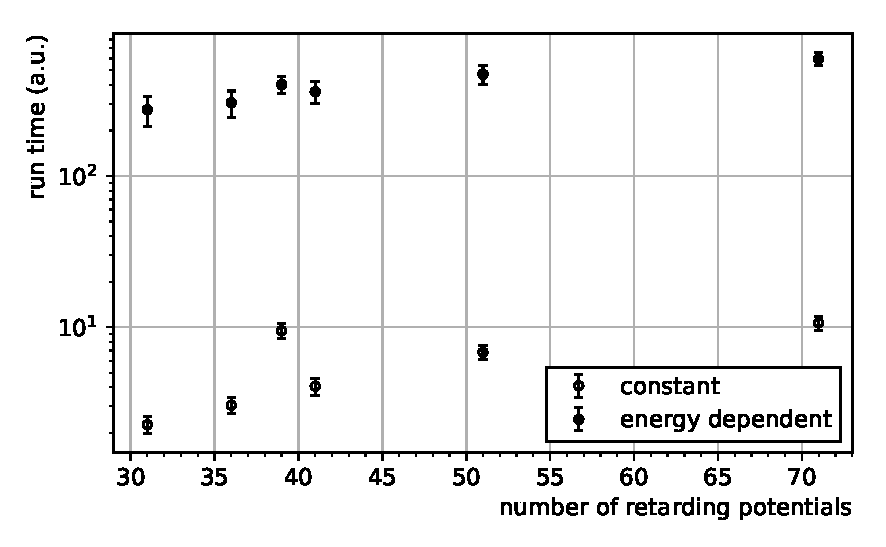
\includegraphics[width=\textwidth]{\currentFigureFolder/scatCrossSecRunTime.pdf}
    \xcaption{Run-time comparison between using an energy-dependent and -independent inelastic scattering cross section}{Run-time comparison between using an energy-dependent and -independent inelastic scattering cross section.}{Shown are the run times for a fit of a simulated model to itself for different \gls{mtd}s. The \gls{mtd}s for the ranges 20, 25, 30, 40 and 50 \SI{}{eV} are taken from the KATRIN design report \cite{Angrik:2005ep} and have a rising number of retarding potentials. A further \SI{90}{eV}-wide \gls{mtd} of the \gls{knm1} campaign was used. It contains 39 retarding potentials. The corresponding run time lies above the trend line as the width of the measurement interval is wider.  For each \gls{mtd} 30 fits were performed. The run times were clocked for a constant and an energy-dependent cross section.}
    \label{fig:scatCrossSecRunTimes}
\end{figure}
The suggested extended model \eqref{eq:energydepScatProbsModel} at its current stage is computationally too expensive to be used in a fitting procedure. Note that a similar model has been derived for a fixed change of the pitch angle $\theta$ per scattering in \cite{Groh2015}. This model for angular changes is implemented in the \gls{ssc} software and can be used in fitting procedures. Though, an important difference is that the determination of the count rate requires an integral over the starting energy $\Esource$ in \eqref{eq:countsDependingOnPositionAndPitchAngle}. Hence, the energy dependent scattering probabilities have to be recomputed in every step of the numerical integration. This is not the case for the model considering the angular changes.

Albeit the energy dependent Poisson model might not fully hold in the case of an energy dependent cross section, figure \ref{fig:energyDependentScatProbs} shows that for larger measurement intervals it is more accurate than assuming energy independent scattering probabilities. Hence, it is a reasonable choice to implement the energy dependent Poisson model into the \gls{ssc} software. This was done. As mentioned the energy dependent scattering probabilities have to be recomputed in every step of the numerical integration in \eqref{eq:countsDependingOnPositionAndPitchAngle} over the $\upbeta$ electron energy. The impact on the run time was probed for 5 different \gls{mtd}s. They differ in the amount and range of retarding potentials. Both aspects should influence the run time. The run time should be approximately linear in the amount of retarding potentials. The run time should get longer the wider the range of the retarding potentials is as the numerically evaluated integral over energies in \eqref{eq:countsDependingOnPositionAndPitchAngle} then stretches over a wider range. Figure \ref{fig:scatCrossSecRunTimes} shows that the run times increase by a factor of approximately $40-120$ between assuming a constant cross section and an energy dependent one.

\section{Effect on the Inferred Neutrino Mass}
\label{sec:eDepScatCrossSecNuMassInf}
\subsection{Neutrino Mass Shift within a Standard KATRIN Measurement Interval}
\begin{figure}[t]
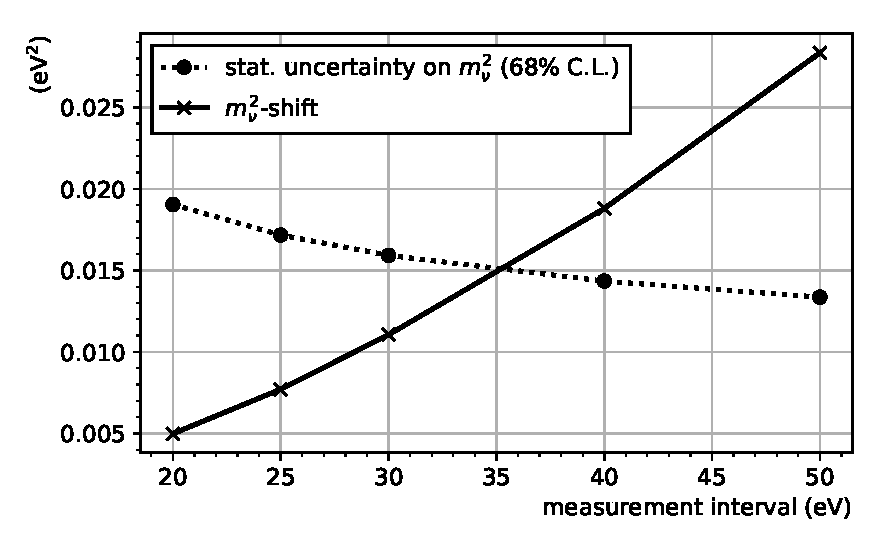
\includegraphics[width=\textwidth]{\currentFigureFolder/effectOnNuMass.pdf}
        \xcaption{Neutrino mass shift due to an energy dependent inelastic scattering cross section}{Neutrino mass shift due to an energy dependent inelastic scattering cross section}{as calculated by SSC for 5 measurement intervals. The configuration for the calculation, especially the \glsentryfull{mtd}, follows the KATRIN Design Report \cite{Angrik:2005ep}. For comparison the statistical uncertainty is plotted as well. It is derived from the profile likelihood. The lines between the 5 markers are linear interpolations.}
        \label{fig:energyDepCrossSecEffectOnNuMass}
\end{figure}
\todo{Numbers can not be reconciled with shifting the cross section. What to do about it?}
In order to determine the influence of the energy dependence of the scattering cross section on the neutrino mass determination the so-called ``shift method'' was used. A description can e.g. be found in \cite{SeitzM2019}. \todo{Write own description} In short, an integrated rate using the energy dependent Poisson model for the scattering probabilities was simulated and fitted to a model using the constant Poisson model. One obtains a deviation of the fitted and simulated neutrino mass, the neutrino mass shift. The procedure was repeated for multiple measurement intervals using the settings from the KATRIN Design Report \cite{Angrik:2005ep} for a 3-year measurement. A comparison of the statistical uncertainty on the neutrino mass and its shift is shown in figure \ref{fig:energyDepCrossSecEffectOnNuMass} depending on the measurement interval. For a measurement interval of approximately \SI{35}{eV} the shift and the statistical uncertainty are approximately equal
\begin{equation}
    \sigma(m_\nu) \approx 
    \sqrt{0.015}\SI{}{eV} = \SI{122}{meV} 
    \text{ (\SI{68}{\percent} C.L.)}
    \fullstop
\end{equation}

\subsection{Neutrino Mass Shift in an Extended  Measurement Interval}
In spring 2019 the so-called \gls{knm1} campaign started. The measurement interval was \SI{90}{eV}. The \gls{mtd} had been optimized according to the up-to-date status of the KATRIN experiment which did not match the KATRIN Design Report in all aspects. The study on the neutrino mass shift was redone scaling the \gls{mtd} of the \gls{knm1} campaign to 3 years and using the corresponding \gls{knm1}-settings. The neutrino mass shift then would be \SI{297}{meV}.


\section{Conclusion and Outlook}
\label{sec:eDepScatCrossSecConclusion}
The energy dependence of the scattering cross section enters into the calculation of the scattering probabilities. An accurate modelling of the energy dependent scattering probabilities is challenging due to performance reasons, but modelling them according to a Poisson distribution is possible. It was shown that the difference between the Poisson model and a more accurate model for 1-fold scattering is on the $10^{-4}$ level. The cases for more than 1 scatterings need further investigation. Also a fixed energy loss per scattering was assumed instead of a energy loss probability distribution. Future work might consider these aspects and what influence a more accurate modeling on the scattering probabilities has on the neutrino mass determination.

Given the KATRIN uncertainty budget, when modeling the energy dependent scattering probabilities via a Poisson distribution, the energy dependence of the scattering cross section is not negligible for measurement intervals that extend more than \SI{35}{eV} below the endpoint of the tritium $\upbeta$ spectrum.

Including the energy dependence in the analysis increases the run time of the fitting procedure significantly. Future work might consider to precalculate the scattering probabilities for different fixed energies and use interpolation techniques for energies in-between the fixed ones.





The total scattering cross section is a sum of the cross section for elastic and inelastic scattering.
\begin{equation}
\sigma(\Ekin) = \sigma_\mathrm{el} + \sigmaInel(\Ekin)
\fullstop
\end{equation}
Only the energy dependence of the inelastic scattering cross section will be considered. This is justified for now as according to \cite{Angrik:2005ep} the cross section for elastic scattering is about an order of magnitude smaller than the one for inelastic scattering. An expression for the inelastic cross section for electrons scattering from hydrogen molecules can be found in \cite{Liu1973}. Two expressions are given, one for relativistic incident particles and one for non-relativistic incident particles. For the maximum relativistic $\beta$ factor of $\upbeta$ electrons from tritium decay one finds
\begin{equation}
\begin{split}
\beta(\Ekin, m) &= 
\sqrt{
	1-\frac{1}{
		(\frac{\Ekin}{m}+1)^2
	}
} \\
\beta_\mathrm{max} &= 
\beta(\Eeff\approx\SI{18.6}{keV}, m_\elecIndex\approx\SI{511}{keV})\approx0.26
\end{split}
\end{equation}
Traveling at approximately a forth of the speed of light, the $\upbeta$ electrons are assumed to be non-relativistic. Then, the given expression for the energy dependent cross section is
\begin{equation}
\label{eq:crossSecLiu}
\sigma(\Ekin) =  
(4 \pi a_0^2) \cdot
\left(\frac{\Ekin}{R}\right)^{-1} \cdot
\left[
C_1 \cdot \ln{\left(\frac{\Ekin}{R}\right)} + C_2
\right]
\end{equation}
with the Bohr radius $a_0$, the Rydberg energy $R$ and two constants given as
\begin{equation}
\label{eq:crossSecLiuConstants}
C_1 = 1.5487 
\quad \text{and} \quad 
C_2 = 2.2212\pm0.0434
\fullstop
\end{equation}
Note that in other works $C_2=2.4036$ \cite{Liu1987} and $C_2=1.53$ \cite{Gerhart1975} are given. The value in \eqref{eq:crossSecLiuConstants} from \cite{Liu1973} was chosen to enable comparability with the KATRIN Design Report \cite{Angrik:2005ep}.

\begin{table}[t]
	\centering
	\xcaption{Inelastic cross section for electrons scattering off molecular hydrogen isotopologues for different incident energies}{Inelastic cross section for electrons scattering off molecular hydrogen isotopologues for different incident energies.}{Listed are important values with reference to KATRIN. Except for the measured value, they are obtained using \eqref{eq:crossSecLiu}. The values are given relative to an assumed endpoint of the measured spectrum $\Eeff=\SI{18575}{eV}$.}
	\begin{tabular}{lll}
		\toprule
		\makecell[tl]{kin. energy} & 
		\makecell[tl]{cross section \\ (\SI{e-22}{m})} & 
		\makecell[tl]{Note} \\
		\hline
		$\Eeff-\SI{1600}{eV}$ & 
		3.740 & 
		largest range in \gls{ft} campaign \\
		$\Eeff-\SI{90}{eV}$ & 
		3.469 & 
		largest range in \gls{knm1} campaign \\
		$\Eeff-\SI{30}{eV}$ & 
		3.459 & 
		KATRIN reference measurement interval \cite{Angrik:2005ep} \\
		$\Eeff-\SI{10}{eV}$ & 
		3.456 & 
		KATRIN reference value \cite{Angrik:2005ep} \\
		$\Eeff$ & 
		3.454 & 
		endpoint of tritium $\upbeta$ spectrum \\
		\SI{18600}{eV} & 
		$3.40\pm0.07$ & 
		measured at the Troitsk experiment \cite{Aseev2000} \\
		\bottomrule
	\end{tabular}
	\label{tab:crossSections}
\end{table}

Furthermore, the total inelastic scattering cross section was measured at the Troitsk experiment and the KATRIN Design Report states a reference value. The values are listed in table \ref{tab:crossSections}. The reference value matches the theoretical calculation using \eqref{eq:crossSecLiu} at a kinetic energy of $\Ekin\approx\SI{18564.4}{eV}$ which would be the center of a $\Delta\Ekin=\SI{20}{eV}$ KATRIN measurement interval. Note that in the KATRIN reference measurement interval $[\Eeff-\SI{30}{eV}, \Eeff]$ the cross section varies  $\sim\SI{0.14}{\percent}$. This variation is below its theoretical uncertainty given by \eqref{eq:crossSecLiuConstants}. In the measurement interval of the \gls{ft} campaign it varies $\sim\SI{8}{\percent}$.



In a KATRIN measurement there exists a minimum retarding energy $\qUmin$ and only electrons with a kinetic energy greater than $\qUmin$ can reach the detector. A scattering cross section averaged over the kinetic energy of the electrons reaching the detector was assumed
\begin{equation}
\sigma = \sigmaAvg = 
\frac{1}{\Delta\Ekin} 
\int_{\qUmin}^{\qUmin+\Delta\Ekin} \sigma(\Ekin) \d \Ekin 
\quad \text{with} \quad
\Delta\Ekin = \Eeff-\qUmin
\fullstop
\end{equation}
Here, the ``effective endpoint'' $\Eeff$ denotes the highest kinetic energy of $\upbeta$ electrons reaching the detector. It does not necessarily match the endpoint of the tritium $\upbeta$ spectrum as experiment specific effects might shift it. $\Eeff=\SI{18575}{eV}$ is assumed. Instead of an average cross section an energy dependent formula can be used. Incorporating the energy dependence makes the model more complicated and slower to compute; neglecting it may lead to wrong results. More light will be shed on both aspects within this chapter.

\section{Motivation and Significance for the KATRIN Experiment}
The motivation to implement an energy dependent cross section into the \gls{ssc} framework is two-fold:
\par{\textbf{Deep scans:} According to \cite{Groh2015} for a neutrino mass determination with the precision goals of KATRIN, the inelastic scattering cross section has to be known with an upper uncertainty of $\SI{0.0055e-22}{m}$ (\SI{0.16}{\percent}). This requirement might be surpassed by neglecting that the scattering cross section is not constant, but varies with energy. According to table \ref{tab:crossSections} the requirement is fulfilled in a measurement interval of $[\Eeff-\SI{30}{eV}, \Eeff]$. According to \eqref{eq:crossSecLiu} it is violated if the lower bound of the measurement interval is below \SI{18531}{eV}. Scans deeper into the tritium $\upbeta$ spectrum increase the count rates and hence, improve the statistic uncertainty on the neutrino mass. Also, for the search of sterile neutrinos deeper scans are necessary. On top of that, deeper scans have already been performed e.g. in the \gls{ft} campaign and help to establish an even better understanding of the KATRIN apparatus. In these cases the energy dependence is not negligible.}
\par{\textbf{Comparability:} A possible cross-check for software is its comparison to other software that was developed independently. \gls{ssc} is part of a data fitting suit. Other fitting software exists within the KATRIN collaboration that uses an energy dependent scattering cross section, e.g. FITRIUM \cite{Fitrium}. Furthermore, \gls{ssc} is commonly cross-checked against a Monte-Carlo particle tracking software called KASSIOPEIA \cite{KATRINCOL2019} which also implements an energy dependent scattering cross section.}


\begin{subequations}
	\label{eq:energydepScatProbsModel}
	\begin{align}
	\mu(E,\thetaSource) =&
	\frac{\sigma(E)\rho L}{\cos\thetaSource} \\
	p_0(E,\thetaSource,n) =&
	\left(
	1-\frac{\mu(E,\thetaSource)}{N}
	\right)^n \\
	p_l(E,\thetaSource,n) =&
	\sum_{k=l}^{n}
	p_{l-1}(E,\thetaSource,k-1)
	\left(
	1-p_0(E-(l-1)\epsilon,\thetaSource,1)
	\right)
	p_0(E-l\epsilon,\thetaSource,n-k) \\
	\bar{p}_l(E,\thetaSource) =& 
	\frac{1}{L}
	\int_{0}^{L}
	p_l(E,\thetaSource,
	\left\lceil N \frac{\zSource}{L}\right\rceil
	)
	\d \zSource 
	\label{eq:energydepScatProbsZAverage} \\
	P^{\star}_l(\Esource,\thetaSource) =& 
	\lim_{N\rightarrow\infty} \bar{p}_l(\Esource,\thetaSource) 
	\label{eq:energydepScatProbsLimit} \\ 
	\bar{P}^{\star}_l(\Esource) =& 
	\frac{1}{1-\cos\thetaMax}
	\int_0^{\thetaMax}
	P^{\star}_l(\Esource,\thetaSource) 
	\d \thetaSource
	\label{eq:energydepScatProbs}
	\fullstop
	\end{align}
\end{subequations}
